\documentclass[11pt, oneside]{article}   	% use "amsart" instead of "article" for AMSLaTeX format
\usepackage{geometry}                		% See geometry.pdf to learn the layout options. There are lots.
\geometry{letterpaper}                   		% ... or a4paper or a5paper or ... 
%\geometry{landscape}                		% Activate for rotated page geometry
%\usepackage[parfill]{parskip}    		% Activate to begin paragraphs with an empty line rather than an indent
\usepackage{graphicx}				% Use pdf, png, jpg, or eps§ with pdflatex; use eps in DVI mode
								% TeX will automatically convert eps --> pdf in pdflatex		
\usepackage{amssymb}
\usepackage{amsmath,amsfonts,amsthm} % Math packages
\usepackage{bm}
\usepackage{graphicx}
\usepackage{dsfont}
\usepackage{pdfpages}
\usepackage{caption}
\usepackage{subcaption}
\graphicspath{ {images/} }

%SetFonts

%SetFonts

\DeclareMathOperator*{\argmin}{arg\,min}
\DeclareMathOperator*{\argmax}{arg\,max}
\newcommand{\horrule}[1]{\rule{\linewidth}{#1}} % Create horizontal rule command with 1 argument of height

\title{	
\normalfont \normalsize 
\textsc{14D006 Stochastic Models and Optimization} \\ [25pt] % Your university, school and/or department name(s)
\horrule{0.5pt} \\[0.4cm] % Thin top horizontal rule
\huge Problemset 2\\ % The assignment title
\horrule{2pt} \\[0.5cm] % Thick bottom horizontal rule
}

\author{Daniel Bestard Delgado, Michael Cameron, Hans-Peter H{\"o}llwirth, Akhil Lohia} % Your name

\date{\normalsize\today} % Today's date or a custom date

\begin{document}
\maketitle


%%%%%%%%
% Problem 1 %
%%%%%%%%
\section{Shortest Path via DP}


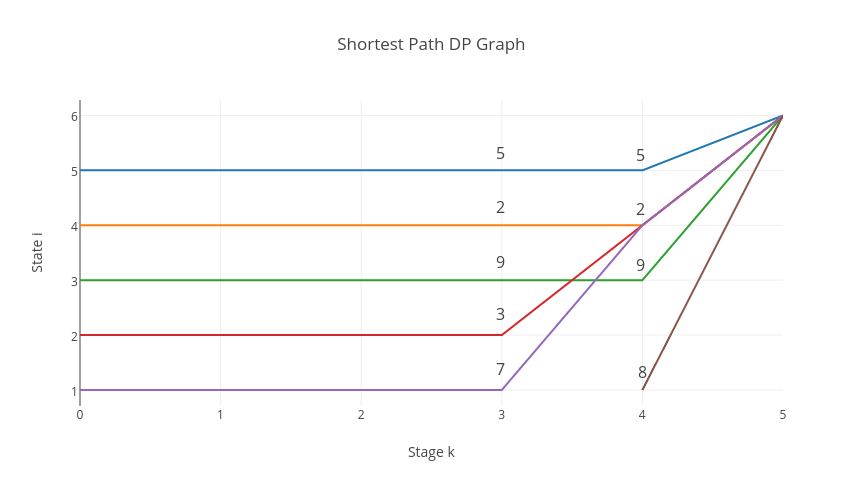
\includegraphics[width=14cm, height=8cm]{Plot2.png} \\
To solve this problem we used the DP set up, where \\
$J_{N-1}(i) = a_{it}, \quad i=1,2,...,N$ \\
$J_{k}(i) = min_{j=1,2,...,6}[a_{ij}+J_{k+1}(j)], \quad k=1,2,...,N-2$  \\

\noindent For example, in this graph, we have $J_{4}(2) = 2$, then following the algorithm \\ $J_{3}(2) = min_{j=1,2,...,6}[a_{2j}+2]=3$. Using this DP algorithm for each node recursively, as discussed in class we find the above graph. Hence the shortest path from each node to node 6 is as follows: \\
From node 1: 7 \\
From node 2: 3 \\
From node 3: 9 \\
From node 4: 2 \\
From node 5: 5


%%%%%%%%
% Problem 2 %
%%%%%%%%
\section{Shortest Path via Label Correcting Methods}
In order to find the shortest path of the directed graph provided in this exercise we need to apply two algorithms that come from the general framework \textbf{label correcting methods}. Before going into detail it is necessary to provide some notation from this general framework:
\begin{itemize}
	\item $i$: denotes the node.
	\item $j$: denotes the child of $i$.
	\item $g_{i}$: length of the shortest path found so far.
	\item $d_{i}+a_{ij}$: length of the shortest path to $i$  found so far followed by arc $(i,j)$.
	\item $UPPER$: length of the shortest path from the source to the target found so far. It is set to $infty$ as long as the target has not been found.
	\item $OPEN$: contains nodes that are currently active, which means that it is possible their inclusion for the shortest path. Initially it contains the source.
\end{itemize}
The label correcting algorithm takes the following steps:
\begin{enumerate}
	\item Remove node $i$ from $OPEN$ and for each child $j$ of $i$, execute step 2.
	\item If $d_{i}+a_{ij} < min\{d_{j},UPPER\}$, set $d_{j} = d_{i}+a_{ij}$ and set $i$ to be the parent of $j$. In addition,
	\begin{enumerate}
		\item If $j \neq t$, place $j$ in $OPEN$ if it is not already in $OPEN$.
		\item If $j = t$, set $UPPER$ to be the new value $d_{i}+a_{ij}$ of $d_{t}$
	\end{enumerate}
	\item If $OPEN$ is empty, terminate; else go to step 1.
\end{enumerate}
One of the algorithms that is part of the label correction methods is the \textbf{Bellman-Ford algorithm}. In this algorithm the node is always removed from the top of $OPEN$ and each node entering $OPEN$ is placed at the bottom of $OPEN$. The following table displays the results of this algorithm for each iteration. Note that in the third column there is a number in parenthesis for each path, which corresponds to its length.
\begin{center}
\begin{tabular}{ | c | c | c | c | }
 Iter. & Exiting OPEN & OPEN at the end of iter. & UPPER\\
 \hline
 0 & - & 1 & $\infty$\\
 1 & 1 & 1-3(1),1-2(2) & $\infty$\\
 2 & 1-2 & 1-2-4(3),1-2-3(3),1-3(1) & 2\\
 3 & 1-3 & 1-3-4(4),1-3-2(2),1-2-4(3),1-2-3(3) & 2\\
 4 & 1-2-3 & 1-3-4(4),1-3-2(2),1-2-4(3) & 2\\
 5 & 1-2-4 & 1-3-4(4),1-3-2(2) & 2\\
 6 & 1-3-2 & 1-3-4(4) & 2\\
 7 & 1-3-4 & $\emptyset$ & 2\\
 \end{tabular}
\end{center}

Just to clarify, note that in the second iteration we reach the target through the path 1-2-5. The length of this path is 2. Given that $j=t$ we set $UPPER$ to be the new value of $d_{t}$ as part b) of the algorithm specifies. The $UPPER$ variable does not get updated anymore because we do not find any other path that goes from the source to the target that has length smaller than 2. Therefore, the shortest path is 1-2-5.\\

The other algorithm that belongs to the label correction methods is called \textbf{Dijkstra's algorithm}. It is very similar to the previous one, but at each iteration it removes from $OPEN$ a node with the minimum value of the label instead of removing the right (top) most node of $OPEN$. The results of the algorithms are:

\begin{center}
\begin{tabular}{ | c | c | c | c | }
 Iter. & Exiting OPEN & OPEN at the end of iter. & UPPER\\
 \hline
 0 & - & 1 & $\infty$\\
 1 & 1 & 1-3(1),1-2(2) & $\infty$\\
 2 & 1-3 & 1-2(2),1-3-2(2),1-3-4(4) & $\infty$\\
 3 & 1-2 & 1-2-3(3),1-3-2(2),1-3-4(4) & 2\\
 4 & 1-3-2 & 1-2-3(3),1-3-4(4) & 2\\
 5 & 1-2-3 & 1-3-4(4) & 2\\
 6 & 1-3-4 & $\emptyset$ & 2\\
 \end{tabular}
\end{center}

Again the shortest path is 1-2-5 for the same reasoning as before. Therefore, both algorithms reach the same outcome in this case.


%%%%%%%%
% Problem 3 %
%%%%%%%%
\section{Clustering}


%%%%%%%%
% Problem 4 %
%%%%%%%%
\section{Path Bottleneck Problem}

\begin{itemize}
	\item $s$: denotes the origin node.
	\item $t$: denotes the terminal node.
	\item $\alpha_{ij}$: length from node i to node j.
	\item $b_{i}$: size of bottleneck in the minimum bottleneck path from s to i.
	\item $p{i}$: parent of node i.
	\item $UPPER$: size of bottleneck in the minimum bottleneck path from s to t. It is set to $infty$ as long as the target has not been found.
	\item $OPEN$: contains nodes that are currently active, which means that it is possible their inclusion for the bottle neck path. Initially it contains the source.
\end{itemize}
The label correcting algorithm takes the following steps:
\begin{enumerate}
	\item Remove node $i$ from $OPEN$ and for each child $j$ of $i$, execute step 2.
	\item If $min\{b_{i},\alpha_{ij}\} < min\{d_{j},UPPER\}$, set $b_{j}=min\{b_{i},\alpha_{ij}\}$, and set $i$ to be the parent of $j$. In addition,
	\begin{enumerate}
		\item If $j \neq t$, place $j$ in $OPEN$ if it is not already in $OPEN$.
		\item If $j = t$, set $UPPER$ to be the new value $d_{i}+a_{ij}$ of $d_{t}$
	\end{enumerate}
	\item If $OPEN$ is empty, terminate; else go to step 1.
\end{enumerate}



%%%%%%%%
% Problem 5 %
%%%%%%%%
\section{TSP Computational Assignment}
We want to find the shortest tour which visits all 734 cities in Uruguay as provided on the website http://www.math.uwaterloo.ca/tsp/world/countries.html. Due to the large number of cities, the DP algorithm is not applicable for this problem. We therefore rely on several heuristic algorithms which approximate the shortest possible path (79,114 km). In particular, we implemented the following algorithms:
\begin{itemize}
\item Nearest neighbor: Select a random city. Find the nearest unvisited city and go there. Continue as long as there are unvisited cities left. Finally, return to the first city.
\item Insert heuristics: Start with random initial subtour consisting of 3 cities. Repeatedly, select a city of shortest distance to any of the cities in the subtour but which is not yet itself in the subtour. Find the shortest detour in the subtour to add this city. Repeat until no more cities remain.
\item 2-Opt Improvement: Take a non-optimal (but valid) path as input. Repeatedly, remove two edges from the tour and reconnect the two paths created (only if the new tour will be shorter). Continue removing and re- connecting the tour until no 2-opt improvements can be found. The tour is now 2-optimal.
\end{itemize}

The resulting tours are as follows (the associated tours are shown in Figure 1):
\begin{itemize}
\item Nearest neighbor: 99,299 km (runtime $<1$ sec)
\item 2-opt nearest neighbor: 86,430 km (runtime $<15$ sec)
\item Insert heuristics: 98,752 km (runtime $<30$ sec)
\item 2-opt insert heuristcs: 89,168 km (runtime $<15$ sec)
\end{itemize}


\begin{figure}[!ht]
\centering
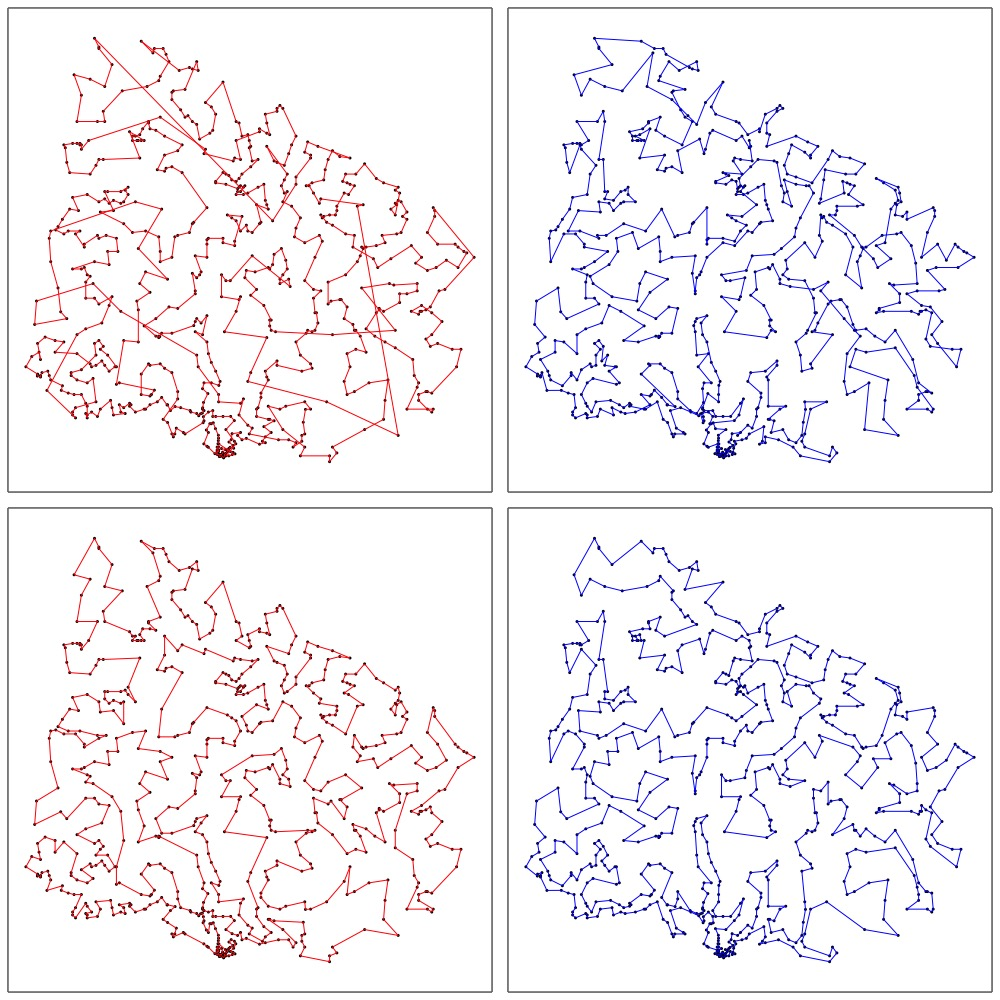
\includegraphics[width=140mm]{images/path-all.jpeg}
\caption{top-left: nearest neighbor tour, bottom-left: 2-opt nearest neighbor tour, top-right: insert heuristics tour, bottom-right: 2-opt insert heuristics tour}
\end{figure} 

\newpage
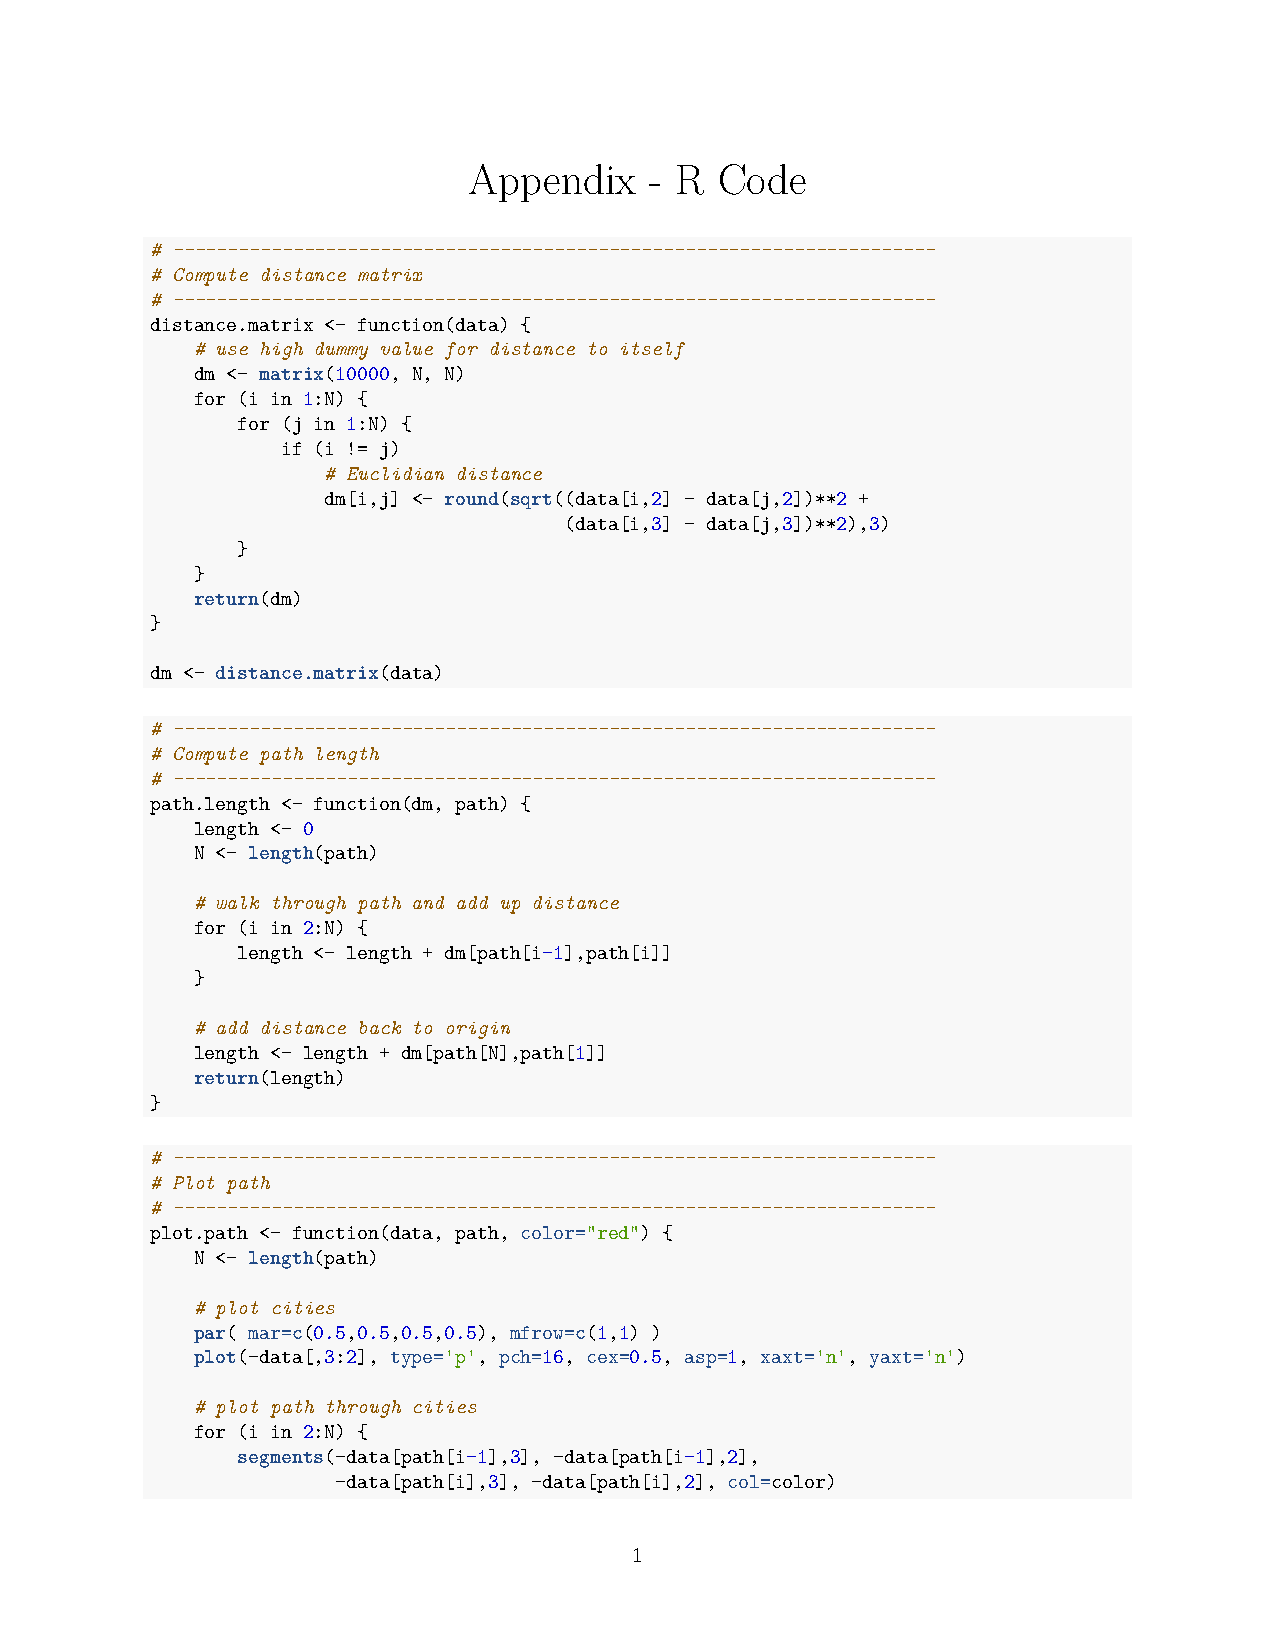
\includepdf[pages={-}]{14D006_MD_PS2.pdf}

\end{document}  















